\documentclass{article}
\usepackage[utf8]{inputenc}
\usepackage{multicol}
\usepackage{amsmath}
\usepackage{float}
\usepackage{epsfig,graphicx}
\usepackage{xcolor,import}
\usepackage{subcaption}
\usepackage[font=small,labelfont=bf]{caption}
\usepackage{siunitx}
\usepackage[german]{babel}
\usepackage{textcomp}
\usepackage{mathtools}

\begin{document}


\thispagestyle{empty}
			\begin{center}
			\Large{Fakultät für Physik}\\
			\end{center}
\begin{verbatim}


\end{verbatim}
							%Eintrag des Wintersemesters
			\begin{center}
			\textbf{\LARGE SOMMERSEMESTER 2015}
			\end{center}
\begin{verbatim}


\end{verbatim}
			\begin{center}
			\textbf{\LARGE{Physikalisches Praktikum II}}
			\end{center}
\begin{verbatim}




\end{verbatim}

			\begin{center}
			\textbf{\LARGE{PROTOKOLL}}
			\end{center}
			
\begin{verbatim}





\end{verbatim}

			\begin{flushleft}
			\textbf{\Large{Experiment 3: Radioaktivität}}\\
							%Experiment Nr. und Titel statt den Punkten eintragen
			\LARGE{}	
			\end{flushleft}

\begin{verbatim}

\end{verbatim}	
							%Eintragen des Abgabedatums, oder des Erstelldatums des Protokolls
			\begin{flushleft}
			\textbf{\Large{Datum:}} \Large{27.03.2015}
			\end{flushleft}
			
\begin{verbatim}
\end{verbatim}
							%Namen der Protokollschreiber
		\begin{flushleft}
			\textbf{\Large{Bachleitner Veronika, Grafendorfer Erik}} 
			\end{flushleft}

\begin{verbatim}


\end{verbatim}
							%Kurstag und Gruppennummer, zb. Fr/5
			\begin{flushleft}
			\textbf{\Large{Kurstag/Gruppe:}} \Large{FR/1}
			\end{flushleft}

\begin{verbatim}






\end{verbatim}
							%Name des Betreuers, das Praktikum betreute.
			\begin{flushleft}
			\LARGE{\textbf{Betreuer: \Large{HUMMER}}}		
			\end{flushleft}
			
\section{Radioaktive Zerfälle}
\begin{center}
\begin{figure}[H]
\begin{subfigure}{0.52\textwidth}
\includegraphics[width=0.9\linewidth]{nuklidkarte.png}
\end{subfigure}
\begin{subfigure}{0.52\textwidth}
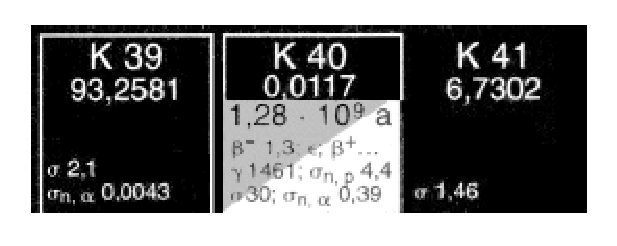
\includegraphics[width=0.9\linewidth]{K-nuklidkarte.eps}
\end{subfigure}
\caption{Links: Gesamte Nuklidkarte, farblich nach Zerfallstyp geordnet (aus Wikipedia: Nuklidkarte); Rechts: Die wichtigsten Kaliumisotope in der Nuklidkarte.}
\label{fig:nuklidkarte}
\end{figure}
\end{center}
Wie in Abbildung \ref{fig:nuklidkarte} zu sehen wird auf der Nuklidkarte nach Protonen- und Neutronenanzahl sortiert. Schwarze Kästchen entsprechen stabilen Isotopen. Ein Isotop unterhalb dieses Bereichs wird durch $\beta^-$-Zerfall ein Neutron in ein Proton umwandeln, bis es zu einem stabilen Nuklid wird.\\
Ein Isotop oberhalb des stabilen Bereichs wird durch $\beta^+$- oder $\alpha$-Zerfall Protonen in Neutronen umwandeln bzw. verlieren, bis es zu einem stabilen Nuklid wird.\\
Zusätzlich kann noch $\gamma$-Strahlung vorkommen, wenn ein Nuklid sich in einem angeregten Zustand befindet. Um auf einen niedrigeren Energiezustand zu fallen wird ein Photon emittiert, das "$\gamma$-Quant". \\
\\
Zur $\alpha$- und $\gamma$-Strahlung wollen wir nicht zu viele weitere Worte verlieren, da im Anleitungstext bereits das wichtigste zu lesen ist.\\
Den $\beta$-Zerfall wollen wir allerdings anhand von Abbildung \ref{fig:beta} genauer beschreiben.\\
\\
Im $\beta^+$-Zerfall (a) wandelt sich durch Emission eines $W^+$-Bosons ein up- in ein down-Quark um. Das $W^+$-Boson zerfällt weiter in ein Positron ($e^+$) und ein Elektron-Neutrino ($\nu_e$). \\
Im $\beta^-$-Zerfall (b) wandelt sich durch Emission eines $W^-$-Bosons ein up- in ein down-Quark um. Das $W^-$-Boson zerfällt weiter in ein Elektron ($e^-$) und ein Elektron-Antineutrino ($\bar{\nu}_e$). 

\begin{center}
\begin{figure}[H]
\begin{subfigure}{0.5\textwidth}
\includegraphics[width=0.6\linewidth]{betaplus.eps}
\caption{$\beta^+$-Zerfall}
\end{subfigure}
\begin{subfigure}{0.5\textwidth}
\includegraphics[width=0.6\linewidth]{betaminus.eps}
\caption{$\beta^-$-Zerfall}
\end{subfigure}
\caption{Feynman-Diagramme von $\beta^+$- und $\beta^-$-Zerfall.}
\label{fig:beta}
\end{figure}
\end{center}

\subsection{Aufgabe: Körpereigene Radioaktivität}
\textbf{Wir schätzen die körpereigene Radioaktivität mithilfe der Nuklidkarte ab.}\\
\\
Wir haben $140g$ Kalium im Körper (ausgehend von $70kg$ Körpergewicht).
Davon sind
$$
140g\cdot 0.000117=1.638\cdot10^{-2}g \\
$$
Kalium 40.\\
Kalium40 hat $40\frac{g}{mol}$. Also haben wir \\
$$4.095\cdot10^{-4}mol$$ Kalium 40 im Körper.\\
\\
Wenn wir dies mit der Avogadro-Konstante multiplizieren erhalten wir:\\
$$2.46607\cdot 10^{20}$$ Atome Kalium 40.\\
\\
Mit einer Halbwertszeit von $T_{\frac{1}{2}}= 1.28 \cdot 10^{9}a=4.039\cdot 10^{16}s$ \\
bekommen wir die Lebensdauer $$\tau=\frac{T_{1}{2}}{\log{2}}=\lambda^{-1} \Rightarrow \lambda=1.7159 \cdot 10^{-17}$$
\\
Daraus gelangen wir schließlich zu dem Ergebnis, dass die körpereigene Aktivität folgenden Wert hat:
$$\boxed{A=N\cdot \lambda = 4.2317\cdot 10^{3} \textrm{ Ereignisse / Sekunde}}$$

\section{Beta- und Gammaspektroskopie}

\subsection{Szintillationszähler}
Der Szintillationszähler wird zur Detektion radioaktiver Strahlung und Röntgenstrahlung verwendet. Die Strahlung erzeugt im Szintillator durch stimulierte Emission Photonen aufgrund der Wechselwirkung zwischen Strahlung und Materie (Photoeffekt, Comptoneffekt und Paarbildung). Die Photonen werden an einer Photokathode in elektrische Ladungen umgewandelt und durch Verstärkung des entstehenden elektrischen Stroms kann die Energie der einfallenden Strahlung gemessen werden.\\
Genauere Informationen sind dem Anleitungstext zu entnehmen.

\subsection{Gammaspektrum}
Da es sich bei unseren Messungen rein um Gammaspektren handelt, werden wir die Betaspektren nicht diskutieren. 
\begin{center}
\begin{figure}
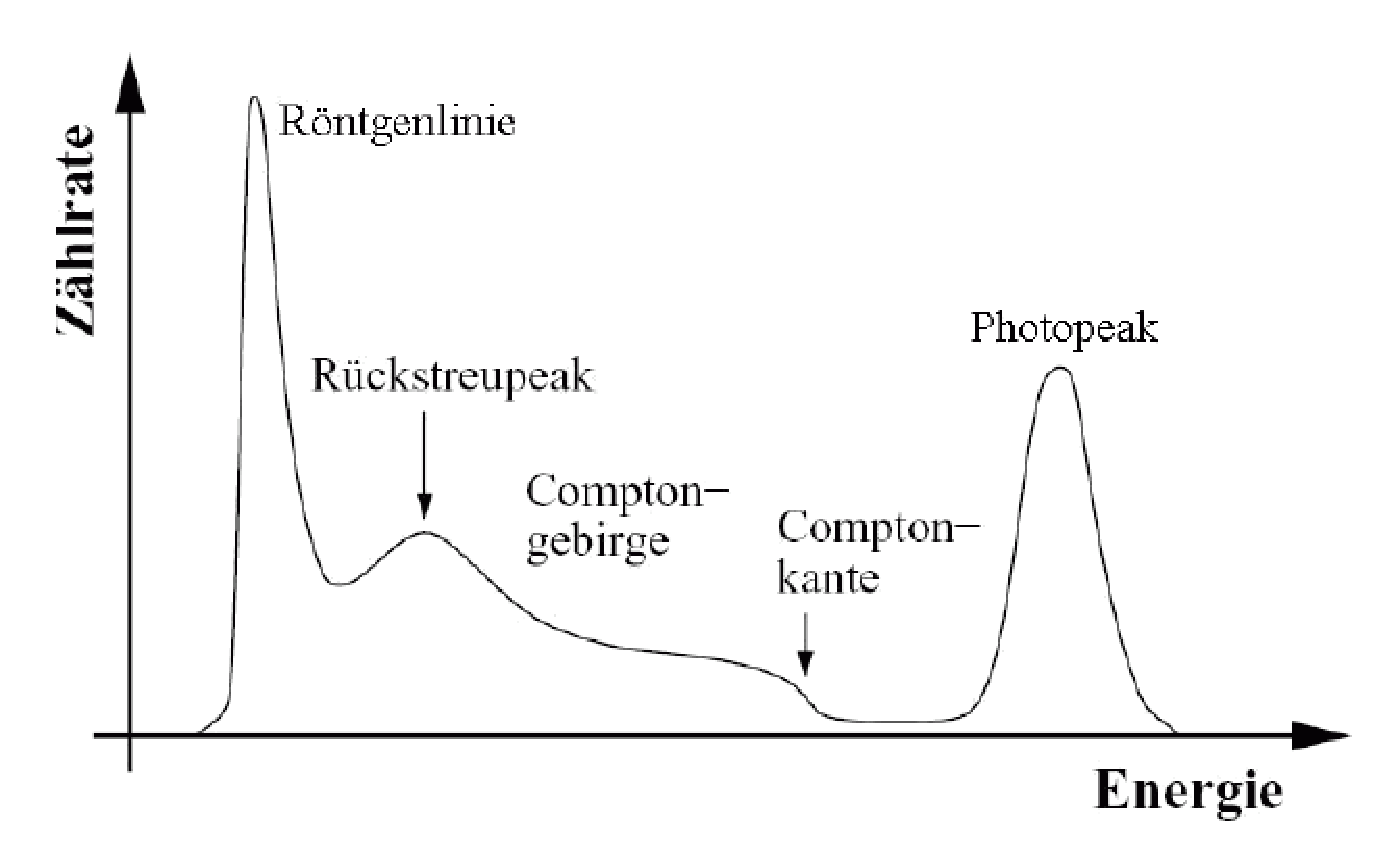
\includegraphics[scale=0.4]{gammaspektren.eps}
\caption{Gammaspektren}
\end{figure}
\label{fig:gamma}
\end{center}
Wie in Abbildung \ref{fig:gamma} zu sehen, gibt es mehrere Peaks in einem Gammaspektrum. Der Verlauf ergibt sich aufgrund der Wechselwirkungen der Photonen mit dem Szintillationskristall. So entstehen Röntgenlinie, Rückstreupeak, Comptongebirge und Comptonkante. Der Photopeak (oder mehrere davon) ist die Energie, die uns eigentlich interessiert. 

\subsection{Aufnahme und Analyse der Spektren}
Zuerst wird eine Aufnahme des Spektrums von Natrium 22 gemacht, auf die die Energie-Skala kalibriert wird. An dieser Skala können die Photopeak-Energien der uns unbekannten Probe abgelesen und das Isotop so bestimmt werden.\\
\\
Anschließend wird das Abstandsgesetz $I(r)\propto\frac{1}{r^2}$ verifiziert.

\subsection{Ergebnisse: Szintillationszähler}
Wir führen eine Messung der Hintergrundstrahlung durch, die wir anschließend nicht von den Messungen der Proben abziehen, da sie so gering und daher vernachlässigbar ist.\\
\\
Bei der Messung von Natrium 22 sehen wir Peaks bei $(513.10 \pm 5.00)\si{keV}$ und $(1275.97 \pm 27.80)\si{keV}$. Die Skala wird auf diese Energien kalibriert.\\
\\
Nachdem eine unbekannte Probe in den Behälter gegeben wurde messen wir wieder und sehen nun Peaks bei $(1181.16 \pm 7.90)\si{keV}$ und $(1333.78 \pm 14.29)\si{keV}$.\\
Aufgrund der gemessenen Peaks stellen wir fest, dass es sich bei der unbekannten Probe um \textbf{Cobalt 60} handeln muss.

\begin{center}
\begin{figure}[H]
\begin{subfigure}{0.52\textwidth}
\includegraphics[width=0.9\linewidth]{bachgrafbild.jpg}
\caption{}
\end{subfigure}
\begin{subfigure}{0.52\textwidth}
\includegraphics[width=0.9\linewidth]{bachgrafunbekannt-peaks.eps}
\caption{}
\end{subfigure}
\caption{Die rote Linie in (a) sowie (b) ist das Gammaspektrum von Natrium 22. Die violette Linie in (b) repräsentiert Cobalt 60. Die horizontale Achse zeigt die Energie, die vertikale Achse die Zählrate.}
\label{fig:szint}
\end{figure}
\end{center}
% -- \ref{fig:name}
In Abbildung \ref{fig:szint} sieht man bei Natrium 22 (a) zwei schöne Photopeaks bei den erwarteten Energien von $(513.10 \pm 5.00)\si{keV}$ ($511\si{keV}$) und $(1275.97 \pm 27.80)\si{keV}$ ($1275\si{keV}$). Auch das Comptongebirge ist gut zu sehen; die Comptonkante befindet sich kurz vor dem zweiten Photopeak. Es gibt auch einen etwas kleineren Peak, der die Röntgenlinie darstellt, sowie einen Rückstreupeak ganz am Anfang des Spektrums.\\
In (b) bei Cobalt 60 ist ganz Ähnliches zu sehen. Es handelt sich hier wieder um zwei Photopeaks bei den erwarteten Energien von $(1181.16 \pm 7.90)\si{keV}$ ($1173\si{keV}$) und $(1333.78 \pm 14.29)\si{keV}$ ($1333\si{keV}$).

\subsection{Ergebnisse: Abstandsabhängigkeit}
%N4:131.44mm : 187 :
%N5:127.30mm : 178 :
%N6:123.22 : 199 :
%N7:115.00 : 209 :
%N8:98.50 :260 :
%N9:65.7 : 479 Ereignisse:
Die Zählrate $Z$ wurde mit dem Szintillationszähler in Abhängigkeit des Abstands von der Strahlungsquelle gemessen.\\
Den Abstand $x$ messen wir mit einer Messlehre; der reale Abstand von der Probe ist $d=x-1$.\\
\\
Da wir die Unsicherheiten der Zählraten nicht mitgeschrieben haben, vergleichen wir mit den Ergebnissen von anderen Mitstudenten. Wir sehen dort relative Unsicherheiten von bis zu $8\%$ und verwenden diese.
\\
\begin{center}
\begin{tabular}{|r|r||l|}
\hline
$x$ ($\si{mm}, \pm 0.01$) & $d$ ($\si{mm}, \pm 0.01$) & $Z$ ($1/s, \pm 8\% $)\\
\hline
$127.30$ & $126.30$ & $178$\\
$123.22$ & $122.22$ & $199$\\
$115.00$ & $114.00$ & $209$\\
$98.50$ & $97.50$ & $260$\\
$65.72$ & $64.72$ & $479$\\
\hline
\end{tabular}
\end{center}

\begin{center}
\begin{figure}[H]
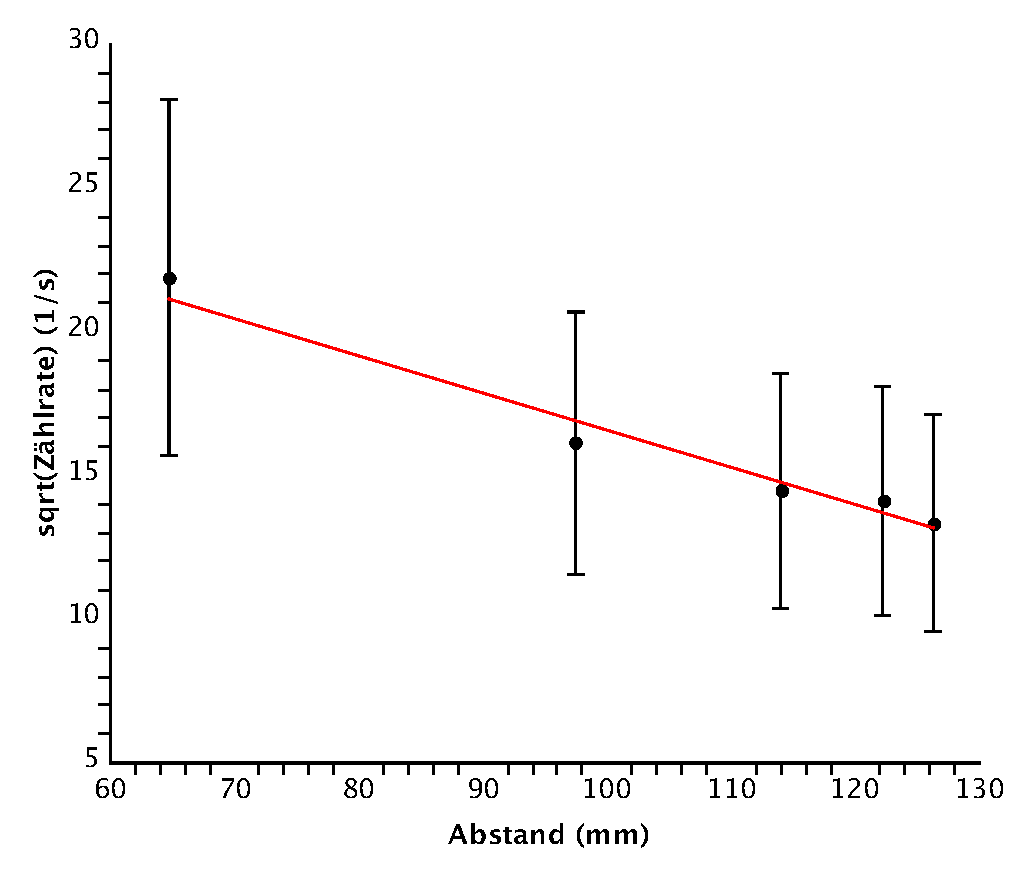
\includegraphics[scale=0.6]{abstandwurzel.eps}
\caption{Linearer Fit zur Abstandsabhängigkeit. Es wurde die Wurzel der Peak-Maxima genommen, um den linearen Fit machen zu können.}
\end{figure}
\end{center}

\section{Nebelkammer}
\section{Geiger-Müller-Zählrohr}																							
\end{document}
